\chapter{Fibre Growth for WM numerical phantom generation}
\label{chap:ipmi-implementation}

\chaptertoc{}

\begin{chapterabstract}
  This chapter introduces a preliminary fibre growth algorithm (\acused{preFiG}\ac{preFiG}), a method for generating \acf{WM} numerical phantoms with realistic orientation dispersion and packing density.
  The growth algorithm is introduced, describing how each \ac{WM} fibre is grown individually to generate a densely packed substrate.

  Some experiments are presented, one of which explores how different inputs to \ac{preFiG} impacts the shape of resulting fibres.
  An application of the method to dMRI is demonstrated with simulations of the diffusion-weighted MR signal in three example substrates with differing orientation dispersions, packing densities and permeabilities.
\end{chapterabstract}


\section{Introduction}
\label{sec:Introduction}
Numerical phantoms have found much use for validating many magnetic resonance imaging (MRI) experiments.
In particular, numerical phantoms are often used when developing diffusion MRI (dMRI) microstructure imaging techniques where simulations of the dMRI signal in phantoms with known microstructural properties are used in lieu of an in vivo ground truth measure of microstructure \cite{Alexander2017}.

While recently numerical phantoms have proven useful for validating microstructure imaging of grey matter \cite{Palombo2020}, they have more commonly been used for validating white matter (WM) microstructure, with many studies comparing parameter estimates from fitting their models to the known ground truth from the phantoms e.g. \cite{Li2019,Jelescu2017,Scherrer2016,Tariq2016,Daducci2015,Nilsson2017,Xu2014,Zhang2012,Nilsson2010}.
Some recent works directly estimate microstructural features using fingerprinting techniques and machine learning to match simulated signals and the corresponding ground truth microstructure of the numerical phantom to the measured signal\cite{Hill2019,Palombo2018a,Rensonnet2018,Nedjati-Gilani2017}.
As well as affecting the dMRI signal, microstructural features also influence other MR techniques such as susceptibility-weighted imaging \cite{Li2012,Lee2010}.
For instance, Xu et al. \cite{Xu2018} recently used simulations to show that using realistic axonal models rather than simple circular cylinders affects the MR signal.
Therefore, it is important to the MRI community to generate realistic WM numerical phantoms which accurately capture microstructural features in order to get realistic simulated signal.

Generating realistic WM numerical phantoms which accurately capture realistic microstructural features (such as dispersion, undulation, beading, etc.) at high packing densities is a major open challenge for the dMRI community.
While densely packing straight, parallel, fibres is relatively easy, only a few groups have attempted to densely pack irregular, non-parallel, fibres.

The most common approach to this is the packing of fibres into densely packed configurations \cite{Close2009,Ginsburger2018,Ginsburger2019,Rafael-Patino2018}.
The typical approach, as taken in the state-of-the-art MEDUSA algorithm \cite{Ginsburger2019}, is to generate a set of overlapping fibres decomposed into small segments and iteratively refine their positions to remove the overlap between them.
Despite their recent progress, further advance of this class of techniques may be limited, because nature does not create fibres before attempting to pack them together.
Instead, real axons are guided by chemical cues and fit into available space as they grow \cite{Price2017,Lowery2009}.
Mimicking the natural fibre genesis may prove important for building more realistic phantoms.

Here, we propose a completely different strategy: rather than densely `packing' irregular fibres, we `grow' fibres contextually, mimicking natural fibre genesis.
We propose a preliminary fibre growth algorithm (\ac{preFiG}) for the generation of WM numerical phantoms with more realistic orientation dispersion and packing density.
Fibres are grown one-by-one following a cost function which attempts to impose the morphological priors that are input to the algorithm.

The rest of the chapter is organised as follows: \Cref{sec:ipmi_config_description} describes \ac{preFiG}, \Cref{sec:impi_experiments_and_results} details some experiments showing the potential of the algorithm and comparing it to a brute-force approach to fibre growth and \Cref{sec:ipmi_discussion} summarises the contributions and discusses limitations in the preliminary implementation and future work to improve the method.


\section{A preliminary fibre growth algorithm}
\label{sec:ipmi_config_description}
In this section we describe a preliminary fibre growth algorithm (\acs{preFiG}) which grows fibres one-by-one avoiding intersection between fibres whilst attempting to ensure that the resulting substrate has desired morphological input properties such as orientation dispersion, diameter distribution and packing density.

The generation of \ac{preFiG} numerical phantoms happens in three main steps:
\begin{description}
  \item [STEP 1] \label{item:step1} Generate initial growth configuration from user inputs
  \item [STEP 2] Grow the fibres using \ac{preFiG} growth algorithm
  \item [STEP 3] Generate 3D meshes for dMRI simulation
\end{description}

The remainder of this section outlines these steps in further detail, breaking each step down into smaller steps and detailing each one in further detail. 

\begin{figure}[t]
  \centering
  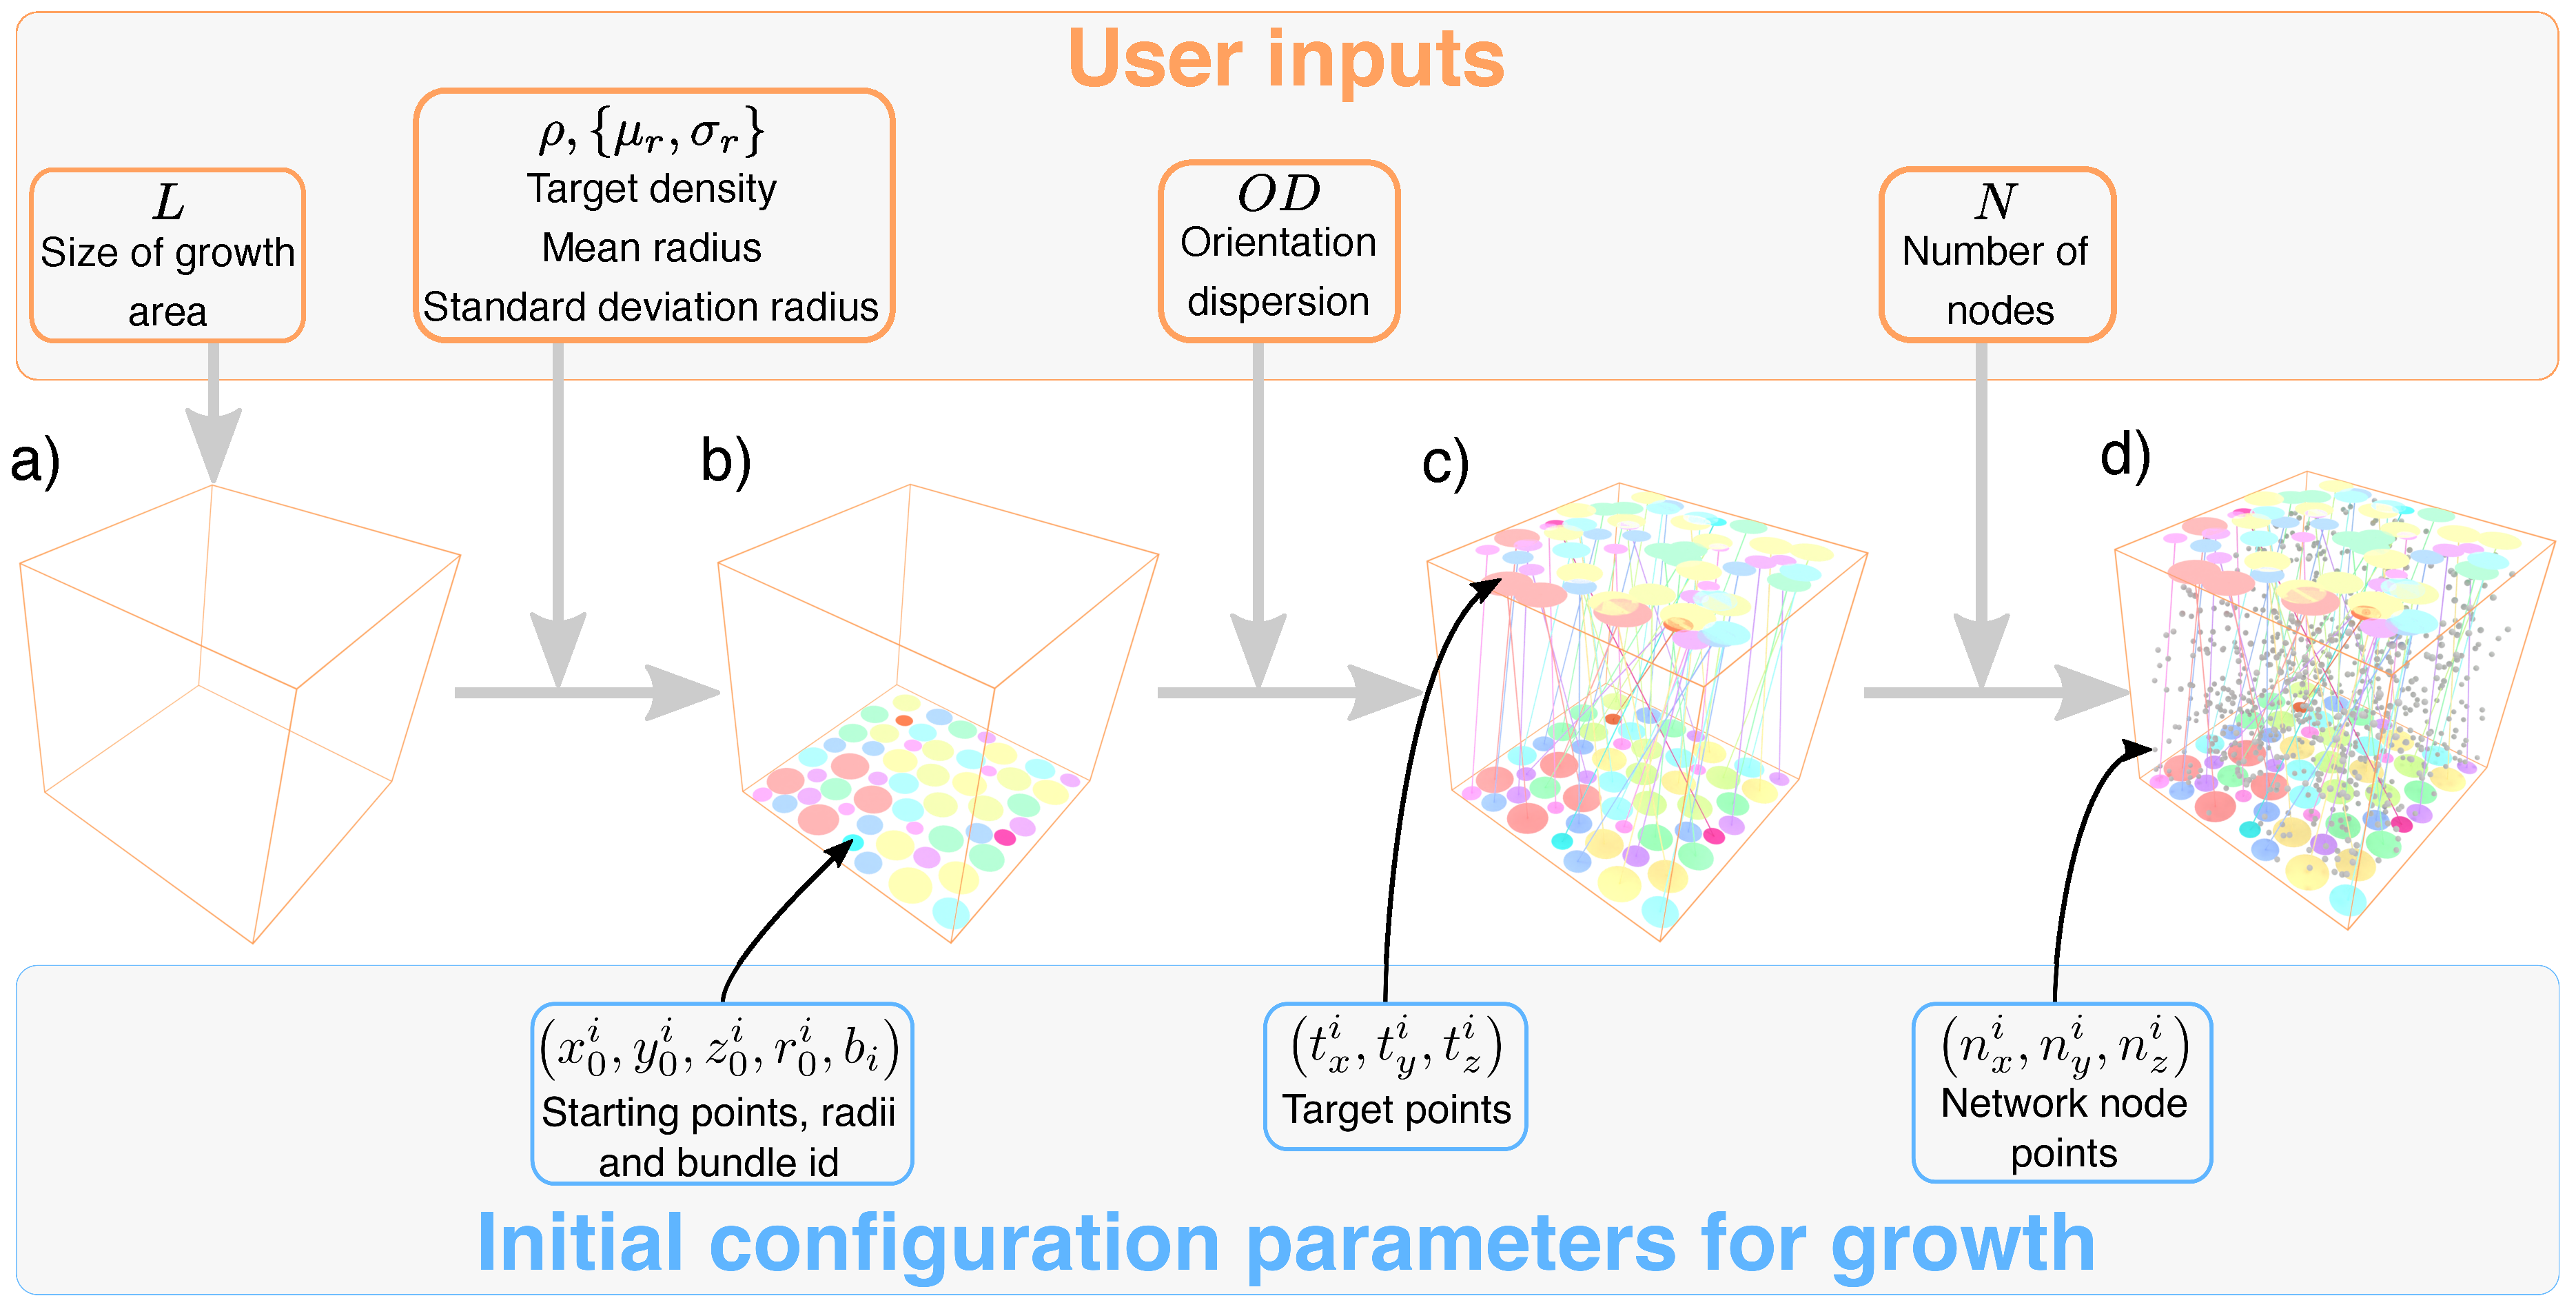
\includegraphics[width=\textwidth]{figures/config/method_inputs_only.eps}
  \caption[Inputs to the \ac{preFiG} algorithm]{Inputs to the \ac{preFiG} algorithm for the single bundle case. $L$ defines the size of the area of that the growth will take place in. The target density and fibre radius distribution govern the generation of starting points for each fibre by packing in 2D. Orientation dispersion parameters govern the generation of target points corresponding to each starting point. $N$ defines the number of nodes to use when generating the network. In the case of multiple bundles, starting and target points are generated for each bundle and then combined into the same space which is filled with nodes for the network. }
  \label{fig:ipmi_inputs}
\end{figure}

\subsection{STEP 1: Initial growth configuration}
\label{sec:ipmi_step1_details}
\textbf{\sffamily STEP 1} is broken down in to three substeps which are outlined in \Cref{fig:ipmi_inputs}:
\begin{description}
  \item [STEP 1.1] Generate fibre starting points for each fibre to grow from (~\Cref{fig:ipmi_inputs}a-b). To generate these starting points \ac{preFiG} packs circles with the desired diameter distribution up to the target density (defined in terms of the desired fibre volume fraction) in 2D, following the approach taken in \cite{Hall2009}.

  \item [STEP 1.2] Generate fibre target points for each point to grow towards (~\Cref{fig:ipmi_inputs}c). To encode the desired orientation distribution, each fibre has a direction drawn from the target distribution which gives a target point for the fibre to grow towards. As a demonstration of the flexibility of the framework, in this work we use the Watson distribution \cite{Mardia2008}.

  \item [STEP 1.3] Generate growth nodes (~\Cref{fig:ipmi_inputs}d). \ac{preFiG} uses a set of pseudorandomly placed points (nodes) to sample the space and encode which regions are occupied by existing fibres. This simplifies collision checking making growth more efficient than a direct collision detection approach involving growing each fibre one small step at a time and checking collisions with existing fibres. This is demonstrated in \Cref{sec:impi_bruteforce}.
\end{description}

\begin{figure}[h!]
  \centering
  \includegraphics[width=\textwidth]{figures/config/method_without_inputs1.eps}
  \caption[Overview of the \ac{preFiG} growth algorithm]{Overview of the basic growth algorithm in \ac{preFiG}. In this example, three fibres are shown with a growth network that only contains relevant nodes for the sake of visualisation.  From the set of nodes, a network is constructed using the Delaunay triangulation. Each fibre then grows from node to node, along any edge connected to the current node. The node moved to will be the node with the lowest cost. Once a fibre segment has grown, the network nodes are updated to store information about which nodes are occupied or near to an existing fibres. This contributes to the cost function for any future fibres, penalising moving to nodes too close to existing fibres.  It is not possible to move to any node now inside a fibre as indicated by the removal of this edges from the network (pairs of blue arrows show where this is happening). The next fibres grow, now avoiding existing fibres until all fibres have finished. See Supplementary Video 1 for an animation of this algorithm. }
  \label{fig:ipmi_config_algorithm}
\end{figure}

\subsection{STEP 2: Fibre growth}
\label{sec:ipmi_step2_growth}
\textbf{\sffamily STEP 2}, the main growth algorithm, is broken down into a series of substeps which are outlined in \Cref{fig:ipmi_config_algorithm}:
\begin{description}
  \item [STEP 2.1] Create growth network (~\Cref{fig:ipmi_config_algorithm}a\&b). In order to encode which nodes a fibre can move to from any other node, the growth nodes are connected using the Delaunay triangulation.

  \item [STEP 2.2] Grow one fibre step (~\Cref{fig:ipmi_config_algorithm}c-e). Fibres grow one-by-one in a random order along this network towards their target points while avoiding existing fibres.

    During growth, a fibre must choose in which direction it should grow. This direction is chosen in \ac{preFiG} by following a cost function which encourages fibres to grow towards their target points (~\Cref{fig:ipmi_config_algorithm}d).
From a starting node, $s$, the candidate nodes, $c$, that the fibre can move to are any nodes that share an edge with $s$. In addition to its position, each network node stores the maximum fibre diameter, $d_c$, that can be sustained at that node without intersecting another fibre (described further in \textbf{\sffamily STEP 2.3}). The fibre will move to a candidate node according to a cost function consisting of two terms; $l_t$, which penalises taking very large steps or moving away from the target point, $t$, and $l_d$, which penalises moving to a position where $d_c$ is low meaning that the fibre will have to shrink. The cost function for a fibre at a position, $s$, to move to a candidate node, $c$, given a target point, $t$, is
\begin{align}
  l &= l_t+fl_d  \,,\label{eq:ipmi_original_cost}\\
      \mathrm{where}\nonumber\\
  l_t &=  \frac{1}{2} \cdot \frac{\|s-c\|}{1+ \|s-c\|} \cdot \left(1- \frac{\left(\left(c-s\right) \cdot \left(t-s\right)\right)}{\|c-s\|\|t-s\|}\right)\,, \label{eq:ipmi_original_lt}\\
  l_d &=\mathrm{max}\left(0, \frac{1}{d_0} \left(d_0 - d_c \right)\right) \,. \label{eq:ipmi_original_ld}
\end{align}
Here, $d_0$ is the target diameter of the fibre and $f$ is a weighting factor between the two terms. In this work, $f$ is fixed to 0.2 to more strongly weight growth towards the target.

The next node for a fibre will be the candidate node which has the lowest cost according to Equation (1). This method of finding a path through the triangulation by choosing the lowest cost node at each position amounts to a greedy best-first pathfinding approach with a heuristic given by Equation (1).

  \item [STEP 2.3] Update the network (~\Cref{fig:ipmi_config_algorithm}f). The growth network is updated in order to store the information about the space this fibre is occupying so that future fibres can avoid it. The way that this is done is to simply store the minimum distance from each node in the network to any existing fibre.

With the next node chosen, the value of $d_c$ needs to be updated for other nearby nodes.
All nodes have $d_c$ set to the Euclidean distance between the node and the surface of the new section of fibre if that distance is less than the current value of $d_c$. This is illustrated in \Cref{fig:ipmi_config_algorithm}d.

Any nodes which now lie within the fibre have $d_c$ set to zero.
Nodes with $d_c = 0$ are disallowed from future steps, meaning that once a fibre has grown, no future fibres can connect to any nodes within the fibre.
This, in addition to shrinking the radius of future fibres according to $d_c$ at each node means that the fibres grow in an almost completely  non-intersecting manner.
Since the value of $d_c$ is set based on fibre-to-point distances, there can be cases in which the fibres would intersect when the closest point between two fibre sections is not at one of the fibre nodes.
In order to account for this, a meshing process developed which can deform fibres around one another. This is described in \Cref{sec:ipmi_step3_meshing}.

  \item [STEP 2.4] Repeat \textbf{\sffamily STEP 2.2} and \textbf{\sffamily 2.3} until fibre reaches target (\Cref{fig:ipmi_config_algorithm}g). By default in \ac{preFiG}, each fibre will grow completely before the next one starts, meaning that \textbf{\sffamily STEP 2.3} only needs to be performed once the fibre has finished growing. If fibres are allowed to grow concurrently, \textbf{\sffamily STEP 2.3} must be performed after each growth step.

  \item [STEP 2.5] Repeat \textbf{\sffamily STEP 2.2-2.4} for remaining fibres (\Cref{fig:ipmi_config_algorithm}h-i). As noted in \Cref{fig:ipmi_config_algorithm} (e-h), as the network is updated, more and more nodes become inaccessible making the network sparser. This means that some fibres may reach a point from which they cannot grow any further and will become stuck. Currently, these fibres are simply removed from the final phantom, meaning the final phantom may have a lower density than the target density.
\end{description}



\subsection{STEP 3: Meshing}
\label{sec:ipmi_step3_meshing}

\begin{figure}
  \centering
  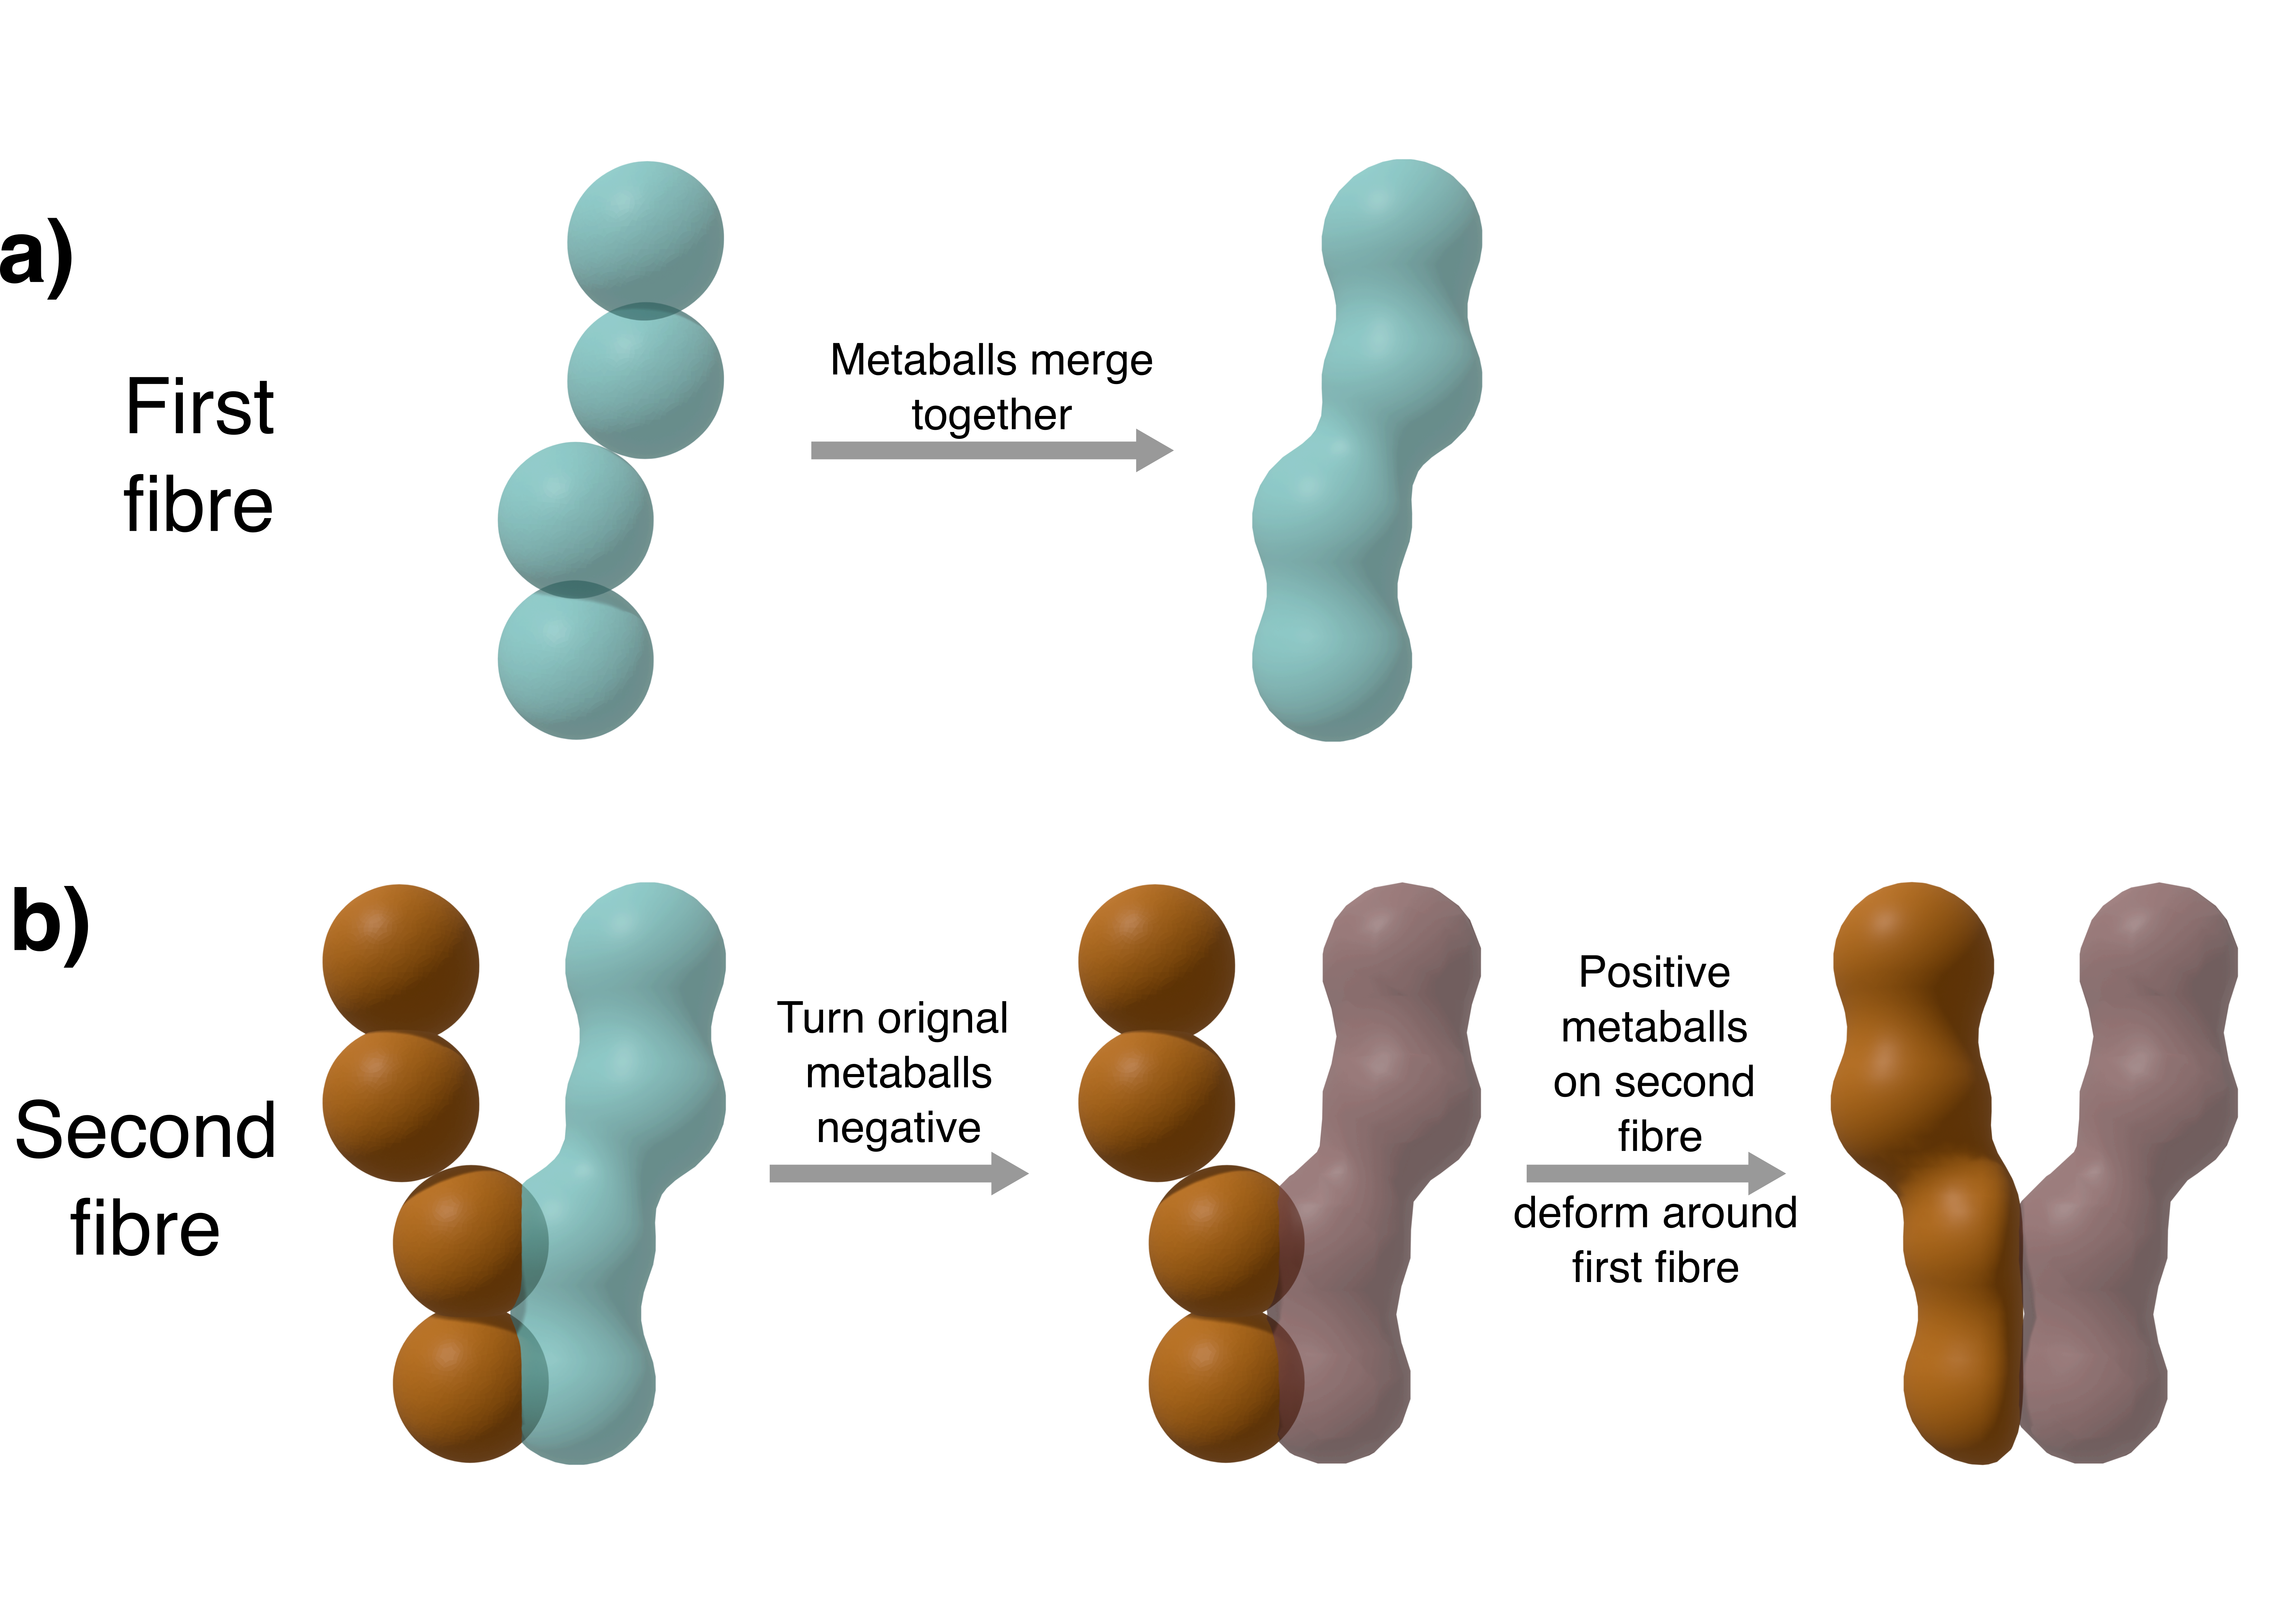
\includegraphics[width=0.8\textwidth]{figures/config/METABALL_fig.png}
  \caption[\ac{preFiG} meshing procedure]{Demonstration of the meshing procedure in \ac{preFiG}. The first fibre is created using metaballs to create a smooth surface. The second, and following fibres will be created using negative metaballs for any fibres that intersect in order to deform around them. Note that in practice, more spheres will be much more closely placed along the skeleton to create a smoother surface}
  \label{fig:ipmi_meshing}
\end{figure}

Finally, \textbf{\sffamily STEP 3}, the meshing procedure is described in more detail below:
\begin{description}
  \item [STEP 3] Generate 3D fibre meshes. After the growth process, each fibre will be represented by a series of connected 3D points and corresponding diameters at each point, stored in the Stockley-Wheal-Cole (SWC) format \cite{Stockley1993}. In order to simulate diffusion MRI signals, these fibre skeleta need to be turned into 3D meshes. \ac{preFiG} uses a meshing procedure designed to eliminate overlap between fibres, using Blender (\url{https://blender.org}), building upon on the SWC mesher addon (\url{https://github.com/mcellteam/swc_mesher}).

\ac{preFiG} meshes are constructed using Blender metaballs, an implicit surface representation which is the isosurface of a function; typically a function analogous to the electric potential from a point charge. When two metaballs come close to one another, the fields combine and the surfaces will merge to form a smooth surface. By placing a series of metaballs along the skeleton of each fibre, a smooth surface is formed for each fibre one-by-one as shown in \Cref{fig:ipmi_meshing}a. Supplementary Figure 1 demonstrates that the \ac{preFiG} meshing procedure does not impact the diffusion dynamics compared to a straight cylinder.

When fibres are densely packed, the surfaces from neighbouring fibres may overlap. To account for this, a meshing procedure was developed in which fibres can deform around nearby fibres to avoid overlap. The metaball surface for one fibre is created as described above. This surface is then turned into a triangulated mesh, however the metaballs are retained. The metaball potential is then turned negative, meaning that rather than merging with any future nearby metaball surfaces, it will repel them, as shown in \Cref{fig:ipmi_meshing}b. This means that subsequent fibres which are meshed very close to, or overlapping with, existing fibres will deform organically to resolve the intersection, thus creating a series of completely non-intersecting fibre meshes which can be used by the dMRI simulator.

\end{description}

% \subsection{Input to the algorithm}
% \label{sec:input}
% The morphology of the final substrate will depend on the inputs to the algorithm which can be split into two general categories: parameters defining the fibre population(s), and parameters defining the space in which fibres grow.

% Fibre parameters include the desired orientation dispersion (OD), packing density ($\rho$) and diameter distribution ($P(d_0)$).
% These three parameters determine the initial settings for each individual fibre.
% Each fibre is defined by a starting point and a target point towards which it will grow as well as an initial fibre diameter, $d_0$.
% These parameters for each fibre are determined from OD, $\rho$ and $P(d_0)$ by packing circles with the diameters drawn from $P(d_0)$ up to a density of $\rho$ in 2 dimensions. Orientation dispersion is introduced by moving the target points of fibres relative to the starting points. %For instance, planar dispersion can be introduced by splitting the substrate into planes and rotating these relative to one another.

% Alternatively, if the user wishes, the starting point, target point and diameter for each fibre can be directly input, rather than allowing \ac{preFiG} to generate them, in order to specify particular fibre configurations such as crossing fibre bundles or fanning fibres.

% Each fibre is allowed to shrink its diameter if it is necessary to fit into spaces close to other fibres.
% The maximum amount of shrinkage permitted is a controllable parameter, specified as a percentage of the initial fibre diameter.

% Due to the stochastic nature of the algorithm, the final substrate is not guaranteed to have the exact morphological properties as input in the priors, however these inputs give the target morphology that \ac{preFiG} will attempt to produce.


% %Parameters defining the space in which the fibres grow are used to define a discretisation of the space which is necessary to make the algorithm run in a practically feasible time.
% %Ideally, the space in which the fibres can grow is a continuous space, so there are an infinite number of positions a fibre can occupy. Practically, this is intractable, so in this algorithm the space is discretised into a set of points which define nodes that the fibres can occupy.

% Parameters defining the space in which the fibres grow are used to define a discretisation of the space into a set of node points that the fibres can occupy. Ideally, the space in which the fibres can grow is a continuous space, so there are an infinite number of positions a fibre can occupy, however this is impractical, so in this algorithm the space is discretised into a finite set of nodes.

% Naturally, the choice of the density and arrangement of node points will impact the substrate that is produced. Too few nodes will result in fibres that have very long, straight segments and may introduce intersections between fibres. Using more nodes will reduce overlap between fibres at the cost of more memory usage and slower growth of the fibres.
% The arrangement of the nodes will also affect the morphology of the final substrate. For instance, placing nodes on a uniform grid may produce fibres with unnaturally angular paths. If the density of nodes on a uniform grid becomes sufficiently high, these angular bends are insignificant compared to the diameter and the fibres will have more natural shapes. For large substrates, the number of nodes required to satisfy this condition becomes intractably large. For this reason, the nodes used are typically pseudo-randomly distributed to ensure broadly uniform coverage of the space, whilst keeping the number of nodes required lower.
% %randomly distributed in the space between the start and target points, to produce more organic shapes whilst keeping the number of nodes necessary lower.

% \subsection{Creation of the Growth Network}
% \label{sec:creation_of_the_growth_network}
% In order to embed information about the local environment at each node, the first step of the algorithm is generating the paths that fibres can take between the nodes as well as defining a maximum diameter that can be sustained at each node to avoid intersection which will be denoted by $d_i$, for a node, $i$. These paths define a network along which the fibres may grow.

% The paths between nodes are defined by the Delaunay triangulation\cite{Delaunay1934} of the nodes which creates a sparse network in which any node can be reached from any other node.
% This triangulation creates edges between nearby nodes, encoding information about the local connectivity at each node.
% Nodes that become occupied by a fibre will be inaccessible to any future fibres, which is one way in which intersection is minimised between fibres.

% The maximum diameter, $d_i$, at each node encodes information on the amount of space available at each node.
% Where $d_i$ is small, that node is close to an existing fibre, so any subsequent fibre passing through that node will have to shrink its diameter to $d_i$ in order to prevent intersections.
% Allowing fibres to contextually shrink their diameter allows fibres to occupy spaces which would otherwise be unavailable.

% \subsection{Growth of a Fibre}
% \label{sec:growth_of_a_fibre}
% \begin{figure}
% 	\centering
% 	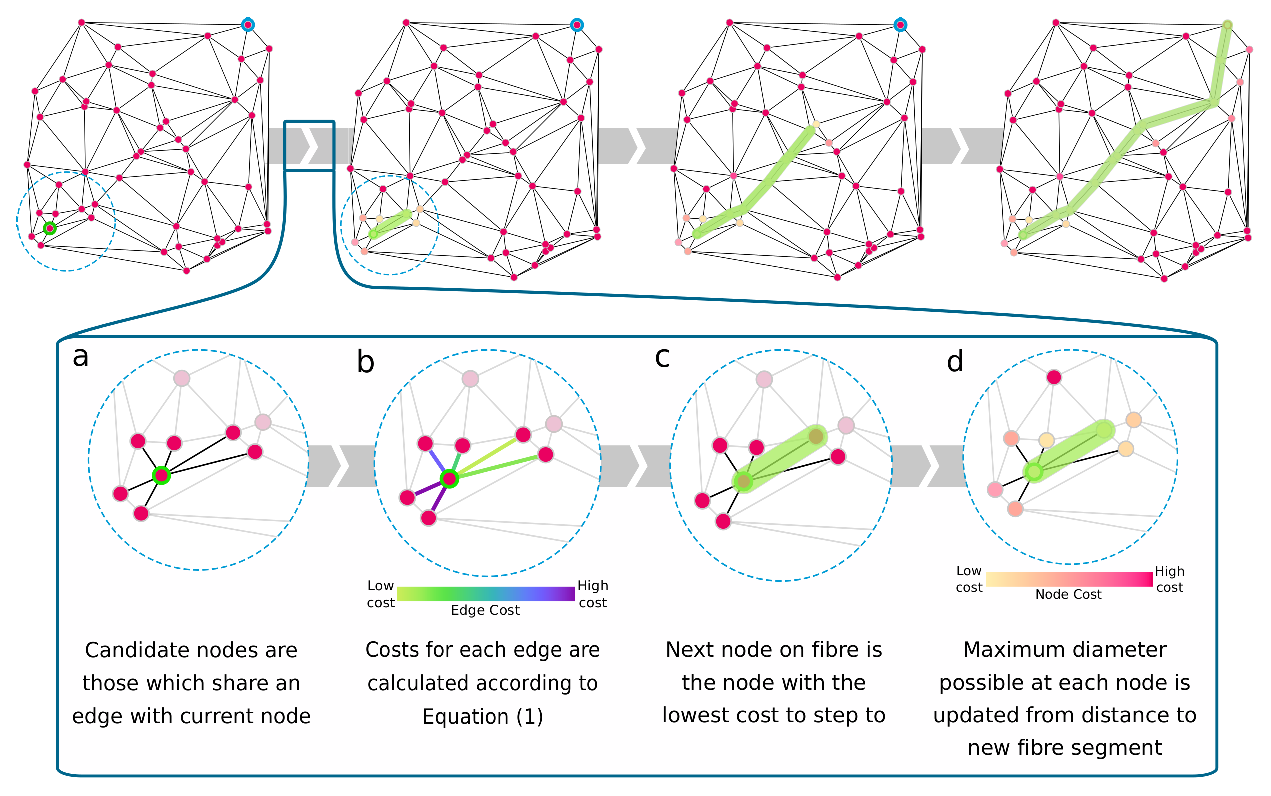
\includegraphics[width = \textwidth]{figures/ipmi_implementation/newMethod_v1.eps}
% 	\caption{\small Schematic overview of the fibre growth algorithm. A fibre grows sequentially, moving from one node to the next, starting from the start point (top left, green node) toward the target (top left, blue node) along the edges defined by the Delaunay triangulation. Inset: The algorithm determining which node a fibre steps to at any given iteration. a) The possible nodes to step to are those which share an edge with the current node. b) From the edges available costs are calculated using \cref{eq:l_t,eq:l_D}. c) The fibre will grow along the edge with the lowest cost. d) From this new segment, the maximum diameter sustainable at a given node is calculated, giving each node a cost based on the maximum sustainable diameter. This cost will then be used in the calculation of edge weights (b) for future fibres. Note that although this figure illustrates the algorithm in 2D, in practice the algorithm grows fibres in 3D.}
% 	\label{fig:method}
% \end{figure}
% Each individual  fibre grows by moving the head of the fibre from node to node according to a cost function which attempts to ensure that the fibre moves towards its target whilst avoiding intersection.
% The main steps in the growth of a single fibre are shown in \Cref{fig:method}.

% The first step in the growth of a fibre is determining which nodes are the possible next nodes the fibre can step to, referred to as candidate nodes.
% From a given starting node, $s$, the candidate nodes are any of the nodes which share an edge with $s$.

% The choice of which candidate node a fibre steps to from the current node is determined by a cost function.
% The cost function consists of two terms, one which penalises moving away from the target point, $t$, and one which penalises moving to a position where $d_i$ is low, meaning the fibre diameter would have to shrink. The cost function for a fibre at a position, $s$, to move to an candidate node, $c$, given a target point, $t$, is $l = l_t + fl_d$,
% % \begin{equation}
% % l = l_t + f l_d\,,
% % \label{eq:costfunction}
% % \end{equation}
% where
% \begin{align}
% l_t &= \frac{1}{2} \cdot \frac{\|s - c\|}{1 + \|s - c\|} \cdot \left(1 - \frac{(c -s)\cdot(t - s)}{\|c-s\|\|t-s\|}\right)\,,\label{eq:l_t}\\
% l_d &= \max\left(0,\, \frac{1}{d_{0}} (d_0 - d_i)\right)\,,\label{eq:l_D}
% \end{align}
% $d_0$ is the desired radius of the fibre and $f$ is a weighting factor between the two terms. In this work, $f$ is fixed to 0.2 to more strongly weight growth toward the target.

% \Cref{eq:l_t} is the term penalising moving away from the target. The dot product between the vector to the candidate and the vector to the target ensures that the minimum cost occurs when the candidate is directly aligned with the target.
% \Cref{eq:l_D} is the term penalising moving to a position where the radius of the fibre must shrink.
% For radii lower than the desired radius of the fibre, $d_0$, \Cref{eq:l_D} grows linearly with distance from $d_0$.
% For radii greater than or equal to $d_0$, \Cref{eq:l_D} is zero, meaning that regions of empty space are equally weighted.

% The next node for a fibre will be the candidate node which has the lowest cost according to \Cref{eq:l_t,eq:l_D}.
% This method of finding a path through the triangulation by choosing the lowest cost node at each position amounts to a greedy best-first pathfinding approach with a heuristic given by \Cref{eq:l_t,eq:l_D}.

% With the next node chosen, the value of $d_i$ needs to be updated for other nearby nodes.
% All nodes have $d_i$ set to the Euclidean distance between the node and the surface of the new section of fibre if that distance is less than the current value of $d_i$. This is illustrated in \Cref{fig:method}d.

% Any nodes which now lie within the fibre have $d_i$ set to zero.
% Nodes with $d_i = 0$ are disallowed from future steps, meaning that once a fibre has grown, no future fibres can connect to any nodes within the fibre.
% This, in addition to shrinking the radius of future fibres according to $d_i$ at each node means that the fibres grow in an almost completely  non-intersecting manner.
% Since the value of $d_i$ is set based on fibre-to-point distances, there can be cases in which the fibres would intersect when the closest point between two fibre sections is not at one of the fibre nodes.
% In order to account for this, a meshing process developed which can deform fibres around one another. This is described in \Cref{sec:creation_of_fibre_meshses}.


% The fibre growth algorithm will output a set of fibres which are defined by a series of nodes and the diameter of the fibre at each node.
% These are written into the Stockley-Wheal-Cole (SWC) format\cite{Stockley1993}, a format commonly used to store cellular morphology information.
% \vspace{-1em}
% \subsection{Creation of Fibre Meshes}
% \label{sec:creation_of_fibre_meshses}
% % \vspace{-0.5em}
% In order to create 3D meshes to be used in dMRI simulations, a meshing process was developed using 3D modelling software Blender (https://blender.org).
% Fibres are meshed one-by-one using the Blender “SWC Mesher” add-on  (https://\\github.com/mcellteam/swc\_mesher) which uses Blender metaballs to make a mesh.

% In Blender, a metaball is an implicit surface defined as the isosurface of a so-called directing structure.
% This directing structure can be seen the source of a static field. For instance a spherical isosurface can be formed with a directing structure which mimics the electric field a point charge.
% When multiple metaballs come close to one another, the fields will combine to form a surface that merges the two spheres together.
% An example of metaball interactions is shown in \Cref{fig:metaballs}.

% By placing metaballs along the skeleton of each fibre, with the path and diameters given from the fibre growth algorithm, a smooth surface is formed for each fibre.
% It is this implicit surface, created using metaballs that the SWC mesher add-on creates.
% This implicit surface can be turned into an explicit surface (i.e. a mesh of vertices and faces) in Blender, which can then be refined by progressively smoothing and reducing the number of faces in the mesh to create a mesh which can be used in dMRI simulations.

% This process can be used to mesh each fibre individually, however issues can arise with intersection of fibres, as mentioned in \Cref{sec:growth_of_a_fibre}.
% In order to account for this, a contextual meshing algorithm was developed.
% The metaball surface for one fibre is created using the SWC Mesher.
% This surface is then turned into a mesh as described above, however the metaballs are retained.
% The metaball potential is then turned negative, meaning that rather than attracting any future nearby metaball surfaces, it will repel them, as shown in \Cref{fig:metaballs}b.
% This means that subsequent fibres which are meshed very close to, or overlapping with existing fibres will deform organically to resolve the intersection, thus creating a series of completely non-intersecting fibre meshes which can be used by the dMRI simulator.

% The deformation introduced by the contextual meshing process has two effects.
% As well as helping to prevent intersection between fibres, the deformation produces fibres with more organic non-circular cross sections, better mimicking realistic mythologies.
% This is vastly different to the majority of previous WM numerical phantoms which model fibres as circular or elliptic cylinders.


% \begin{figure}
%   \centering
%   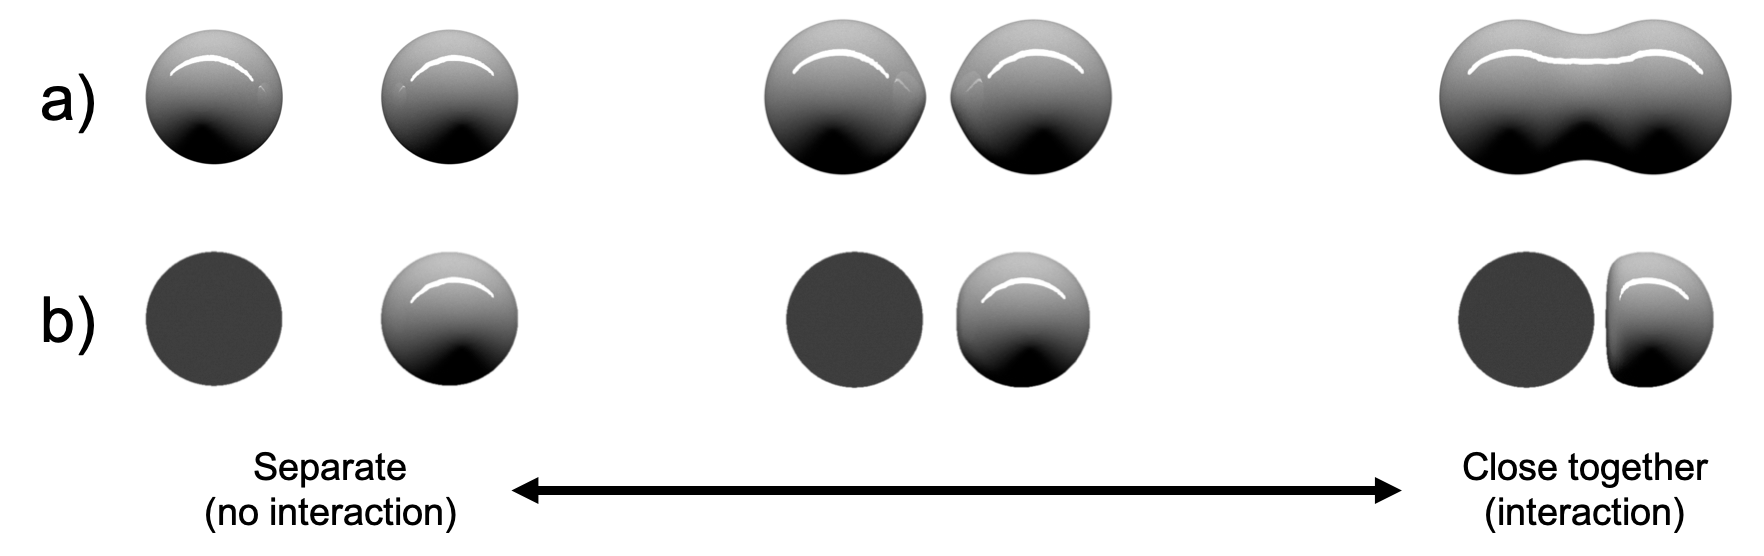
\includegraphics[width=\textwidth]{figures/ipmi_implementation/metaballs.png}
%   \caption{\small Simple example of metaball interactions. a) With two positive metaballs, the fields combine to attract the surfaces together. This is used to join individual segments into a continuous fibre. b) With one negative metaball (indicated by the flat grey circle) the surface of the metaball is repelled from the negative metaball. This is used to deform nearby fibres around one another.}
%   \label{fig:metaballs}
% \end{figure}



\section{Experiments and Results}
\label{sec:impi_experiments_and_results}
\subsection{Effect of choice of growth network}
\label{sec:ipmi_choice_of_network}
\begin{figure}
  \centering
  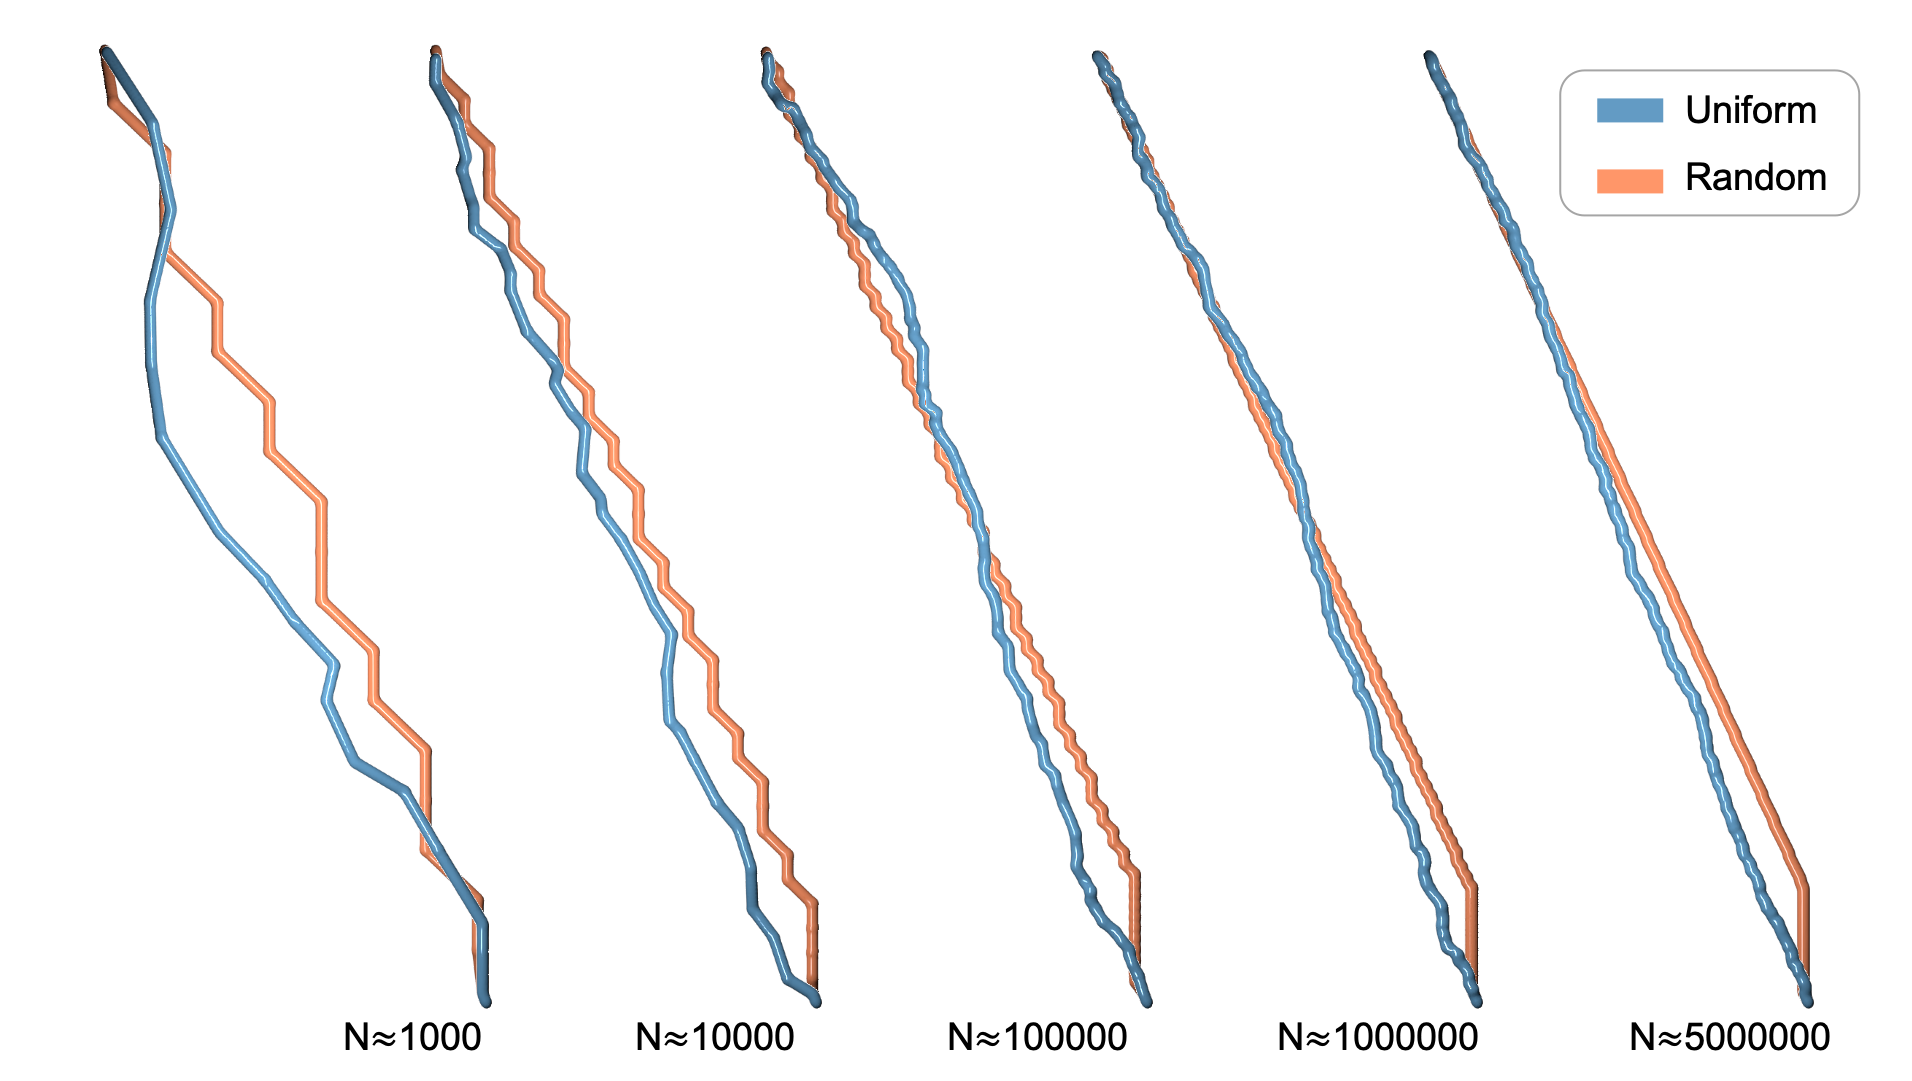
\includegraphics[width=0.9\textwidth]{figures/ipmi_implementation/uniform_vs_rand.png}
  \caption{Fibres generated using uniform grid (orange) and pseudo-random (blue) network nodes for increasing numbers of nodes.}
  \label{fig:ipmi_uniform_vs_rand}
\end{figure}
As mentioned in \Cref{sec:ipmi_step1_details}, the choice of the node points in the network will affect the morphology of the resulting substrate.
In order to investigate this, a qualitative experiment was performed in which a single fibre was grown on a network with either a) nodes on a uniform grid or b) pseudorandom nodes.
In each case, the number of nodes was increased and the resulting fibre investigated.

The fibre was defined by a start point (20, 0, 0) $\mu$m,  target point (0, 0, 50) $\mu$m and diameter 1 $\mu$m.
This configuration was chosen so that the fibre would not have a path that directly followed one of the 90\degree\ or 45\degree\ lines in the uniform grid.
Node points were initialised in either a uniform grid or pseudorandomly within the space [-5, -5, -5] to [25, 5, 55] to ensure coverage of the space in which the fibre would grow.
The number of source points used was $N \approx 1000, 10000, 100000, 1000000, 5000000$.

The resulting fibres can be seen in \Cref{fig:ipmi_uniform_vs_rand}, where orange fibres are grown using the uniform grid and blue fibres using pseudorandom points.
In both cases, as the number of nodes increases, the resulting fibre has more of a smooth, straight path between start and target.
The uniform grid fibres, have a much more angular, structured path due to being forced to grow on the grid, while the pseudorandom fibres more irregular paths, which could be considered more `organic' looking.


\subsection{Demonstration of \acs{preFiG}}
\label{sec:ipmi_demonstration}
To demonstrate the potential of \ac{preFiG}, three substrates at different (dispersion, packing density) conditions were generated: (0\degree, 60\%), (15\degree, 30\%) and (35\degree, 25\%), shown in \Cref{fig:ipmi_substrates_signals}a.
Each substrate is grown using $5 \times 10^6$ pseudo-randomly placed source nodes for the growth network, giving a network with $3.88\times10^7$  edges and a mean distance between any given node and its neighbours of 0.29 $\mu$m.
The packing densities chosen represent the highest densities achievable using \ac{preFiG} for each dispersion condition.


For the 0\degree\ dispersed substrate, initial diameters were drawn from a gamma distribution with mean $d_0 = 2\ \mu$m and standard deviation $\sigma_d = 0.2\ \mu$m. The 15\degree\ and 35\degree\ substrates were generated with $d_0 = 1.2\ \mu$m and $\sigma_d = 0.2\ \mu$m in order to show the flexibility of \ac{preFiG} to generate substrates with different diameter distributions as well as orientation dispersion and packing density. Diameters were limited to be permitted to shrink to 25\% of the original fibre diameter in order to fit into space.

For each substrate, the \acf{PGSE} signal was simulated in Camino\cite{Cook2006} using $5\times 10^5$ diffusing spins and $5\times 10^3$ discrete time steps, uniformly distributed with bulk-diffusivity D$_0$=2 $\mu$m$^2$/ms. To show the range of simulation possibilities available, three different membrane permeabilities ($\kappa$=0, 0.0025, 0.0050 $\mu$m/ms) were also imposed.
The simulated \ac{PGSE} measurement parameters were: $\delta/\Delta=1/40$ ms and 50 b-values from 0 to 9 ms/$\mu$m$^2$ along x-, y- and z-directions.

The corresponding direction-averaged simulated \ac{PGSE} signals at different permeabilities are shown with SNR = $\infty$ in \Cref{fig:ipmi_substrates_signals}b and SNR = 20 in \Cref{fig:ipmi_substrates_signals}c.
The signal decays to a lower value as the dispersion increases and density decreases, as expected.

\begin{figure}[h!]
  \centering
  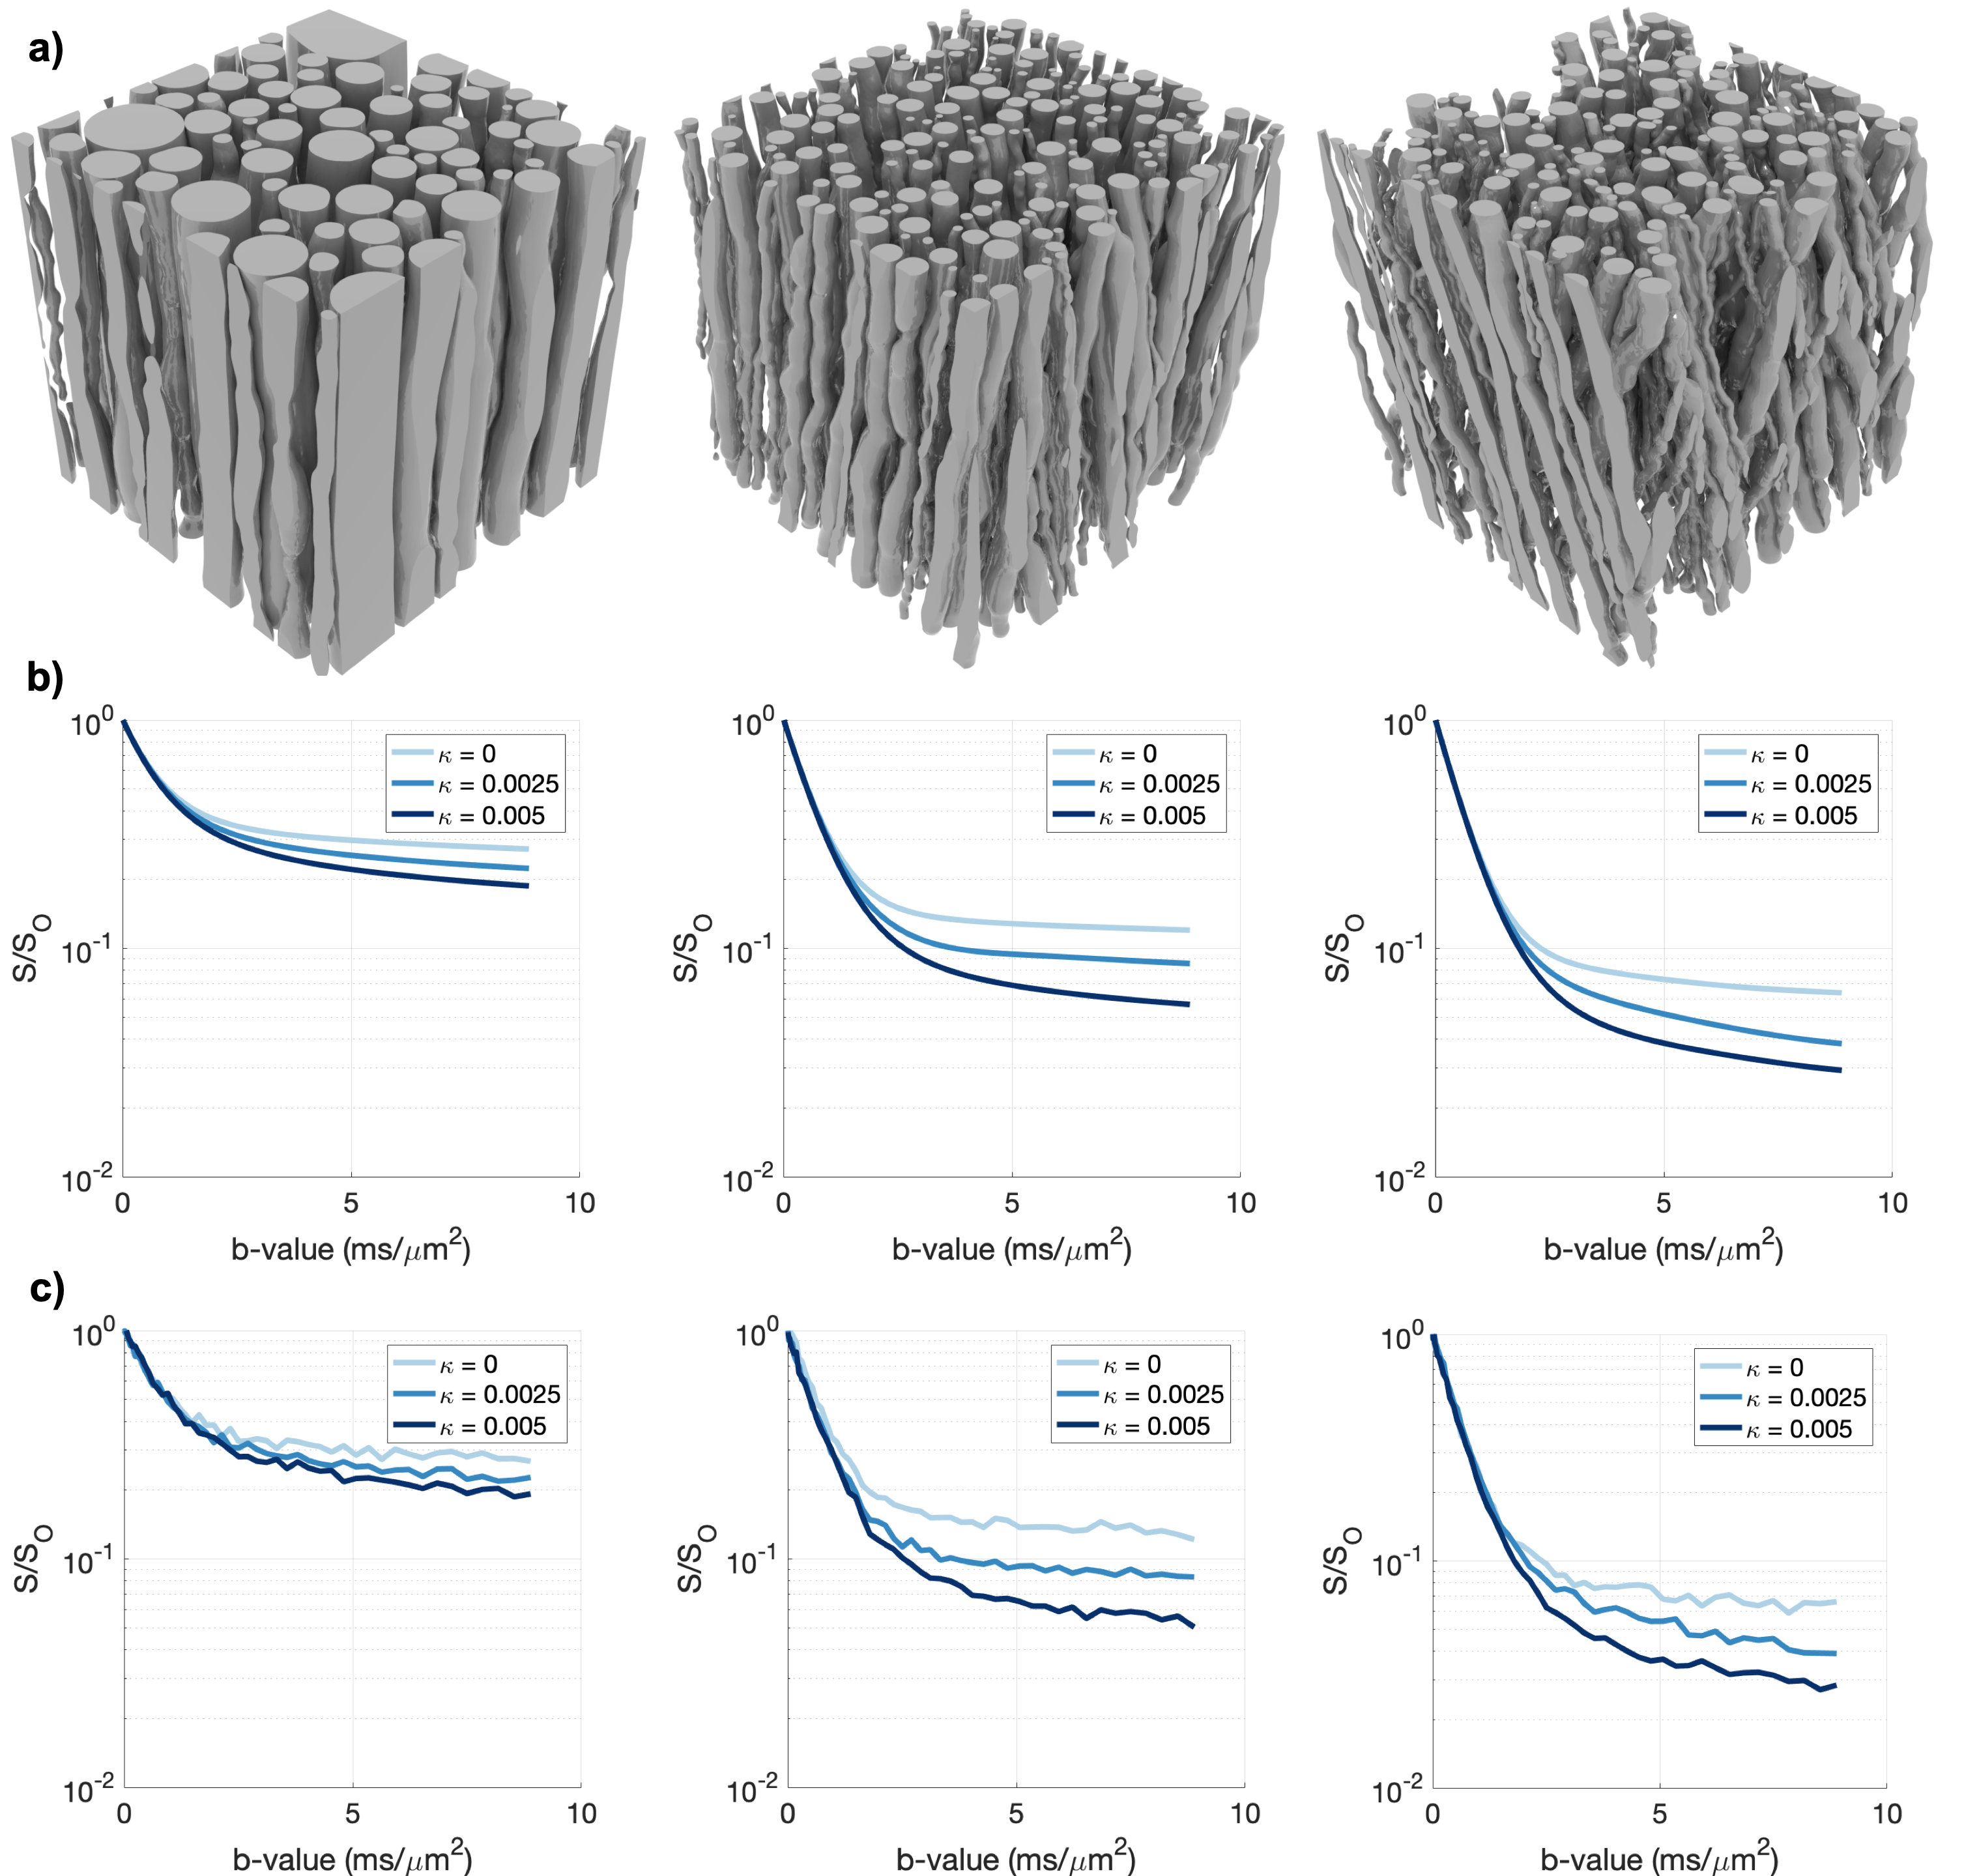
\includegraphics[width=\textwidth]{figures/ipmi_implementation/substrates_and_signals_otherlabels.png}
  \caption[Examples of generate WM numerical phantoms and simulated dMRI signals]{\small a) Example substrates (cut into 30x30x30 $\mu$m$^3$ cube) from the fibre growth algorithm, left to right:  Zero macroscopic dispersion (60\% density), 15\degree\ of macroscopic dispersion (30\% density), 35\degree\ dispersed (25\% density). b) Simulations for each substrate for varying permeabilities with SNR = $\infty$  and c) SNR = 20. Units of $\kappa$ are $\mu$m/ms.}
  \label{fig:ipmi_substrates_signals}
\end{figure}

\subsection{Comparison with brute-force approach}
\label{sec:impi_bruteforce}
\ac{preFiG} was compared against the na\"ive brute-force approach to fibre growth.
The brute-force approach grows fibres one segment at a time and checks for collisions between the new segment and all existing fibres.
Each new segment is chosen from one of 128 candidate directions on a cone aligned with the previous segment, with each direction being weighted according to \Cref{eq:ipmi_original_lt}.
%In the case of collisions between the proposed new section and an existing fibre, each direction is tested in order of the weight of the direction until a non-colliding direction is found, or all directions have been tested and the fibre is stuck.

Substrates were grown with both the brute-force approach and \ac{preFiG} using the same starting and target points and initial diameters.
These initial parameters were determined by packing circles with gamma distributed radii (mean $d_0 = 2\ \mu$m, standard deviation $\sigma = 0.6\ \mu$m) into a 40 $\mu$m x 40 $\mu$m square up to a packing density of 60\%. Target points were set as 40 $\mu$m directly above the starting points to define a substrate with 0\degree\ macroscopic orientation dispersion.
This resulted in a substrate with a total of 54 initial fibres.

The fibre growth algorithm used $1\times 10^6$ randomly distributed points for the Delaunaty triangulation giving a mean distance between points of 0.5 $\mu$m, matching the brute force approach which used a segment length of 0.5 $\mu$m for each new fibre segment.

From these initial parameters, fibres were grown using a subset of $n = 1, 5, 10, 15, 20, 25, 30, 40$ fibres and the growth was timed. Each value of $n$ was timed 5 times with and the mean taken to reduce single-run timing fluctuations.

\begin{figure}[t]
  \centering
  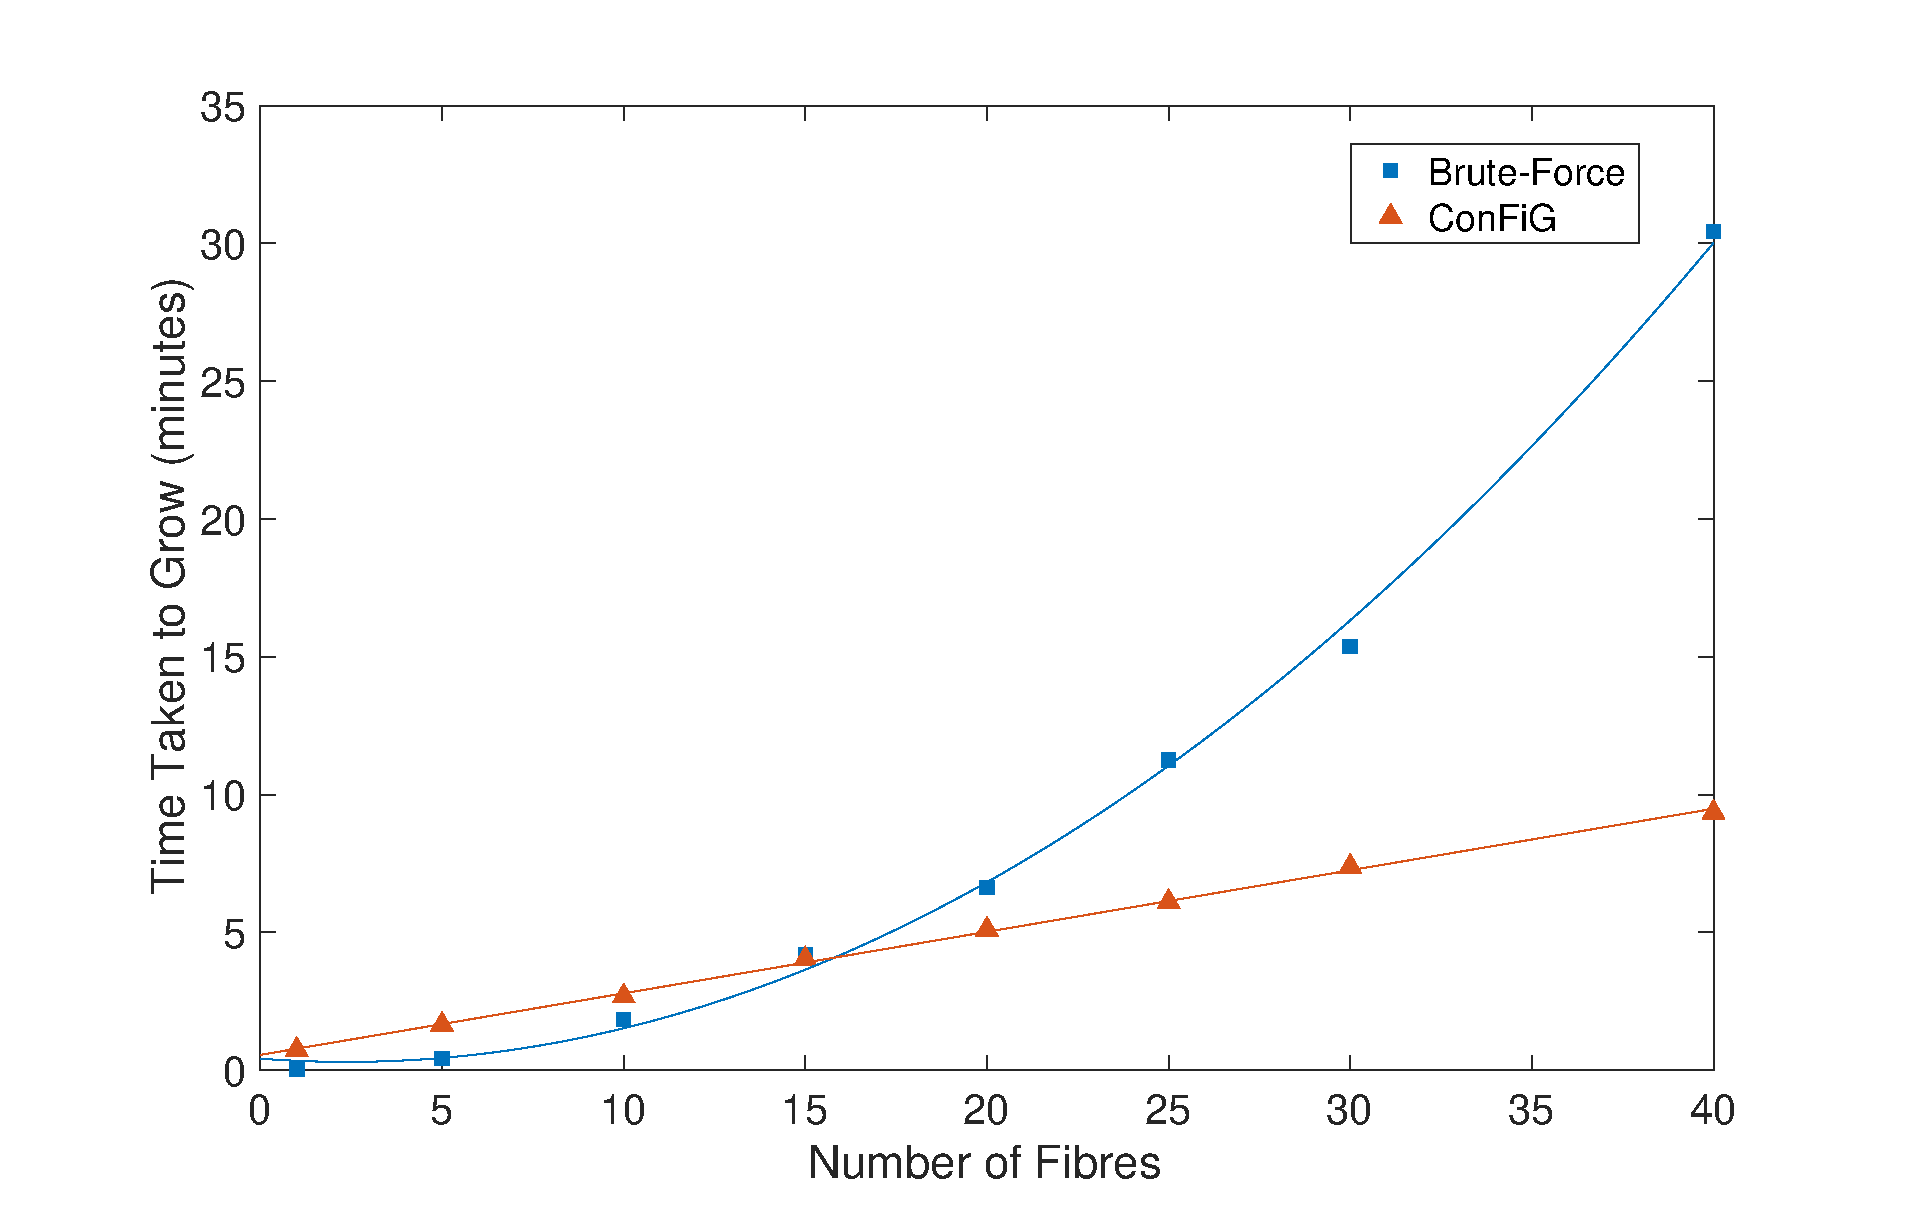
\includegraphics[width=0.8\textwidth]{figures/ipmi_implementation/brute_force_vs_algo_2.eps}
  \caption[Comparison of brute-force growth and proposed fibre growth algorithm]{\small Timing of brute force growth vs.\ the fibre growth algorithm along with a quadratic fit (brute-force) and linear fit (fibre growth algorithm). The fibre growth algorithm is clearly linear in the number of fibres, while brute force growth fits an order $n^2$ well. }
  \label{fig:impi_brute_force}
\end{figure}

\Cref{fig:impi_brute_force} shows the timing results of the brute-force approach versus the fibre growth algorithm.
The fibre growth algorithm  has approximately $\mathcal{O}(n)$ complexity with $n$ being the number of fibres.
Conversely, the brute-force algorithm shows $\mathcal{O}(n^2)$ complexity owing to the fact that every new segment has to check for collisions with all existing fibres.

The fibre growth algorithm has a higher $n=0$ offset which is caused by the overhead in calculating the Delaunay triangulation for the growth network.
This causes the brute-force approach to have better performance at low $n$, while at higher $n$ (approaching the $>100$ fibres needed for a realistic dMRI voxel) the linearity of the fibre growth algorithm gives it much faster performance.



\section{Discussion and Conclusion}
\label{sec:ipmi_discussion}
\ac{preFiG} shifts the perspective from previous works attempting to pack together fibres, by trying to mimic natural fibre genesis.
This approach represents a major step towards very high fibre packing, enabling us to reach the highest dispersion at the highest packing density reached so far, to our knowledge. Our (15\degree, 30\%) and (35\degree, 25\%) represent an average \mytilde50\% and \mytilde200\% improvement, respectively, over the best previously reported results of (10\degree, 20\%)\cite{Ginsburger2018}\footnote{The \ac{preFiG} method presented here outperformed the state-of-the-art at the time it was published \cite{Callaghan2019}}.


The substrates presented in \Cref{fig:ipmi_substrates_signals} are just a few examples of the kinds of substrates that can be produced using our \ac{preFiG} method, though by varying the setup of the morphological controls and start and target points, many different fibre configurations can be produced.
Currently, fibres will attempt to grow in a straight line between the start and target points, meaning that certain configurations such as kissing bundles cannot be represented.
However, the algorithm can in principle be extended to allow for series of target points, allowing the definition of a desired 'path' of a fibre.

Additionally, some input parameter settings cannot be achieved.
For instance, trying to grow a substrate with both very high density and very high dispersion will result in a final substrate that does not reach the density required.
The reason for this could be a combination of limitations of the algorithm in restricting growth to a discrete network and also the fact that some morphological settings are practically infeasible.
This limitation, however, also applies to the fibre packing and  brute force growth approaches.

One weakness of the fibre-growth algorithm is that since the fibre diameters are calculated from a fibre-to-point distance, there can still be some small amount of overlap between fibres.
This is solved using the meshing process in Blender to deform the regions of slight overlap between neighbouring fibres.

Another limitation of the \ac{preFiG} implementation is that while the phantoms produced improve upon the state-of-the-art, the fibre density achieved is still too low to really be applicable to white matter. Typical expected fibre density would be between 50 and 80\%, so improvements need to made to enable phantoms to be generated at a higher fibre density.

To conclude, the proposed \ac{preFiG} approach, using the fully connected growth network, is shown to be more efficient than a `brute-force' growth approach.
The fact that \ac{preFiG} is linear with the number of fibres makes it far more efficient for high numbers of fibres. For instance, a realistic voxel will need hundreds or thousands of fibres which will become impractically slow for the `brute-force' approach, whilst remaining manageable for our algorithm.
This efficiency, along with the high density and orientation dispersion achieved means that \ac{preFiG} represents a promising step forward in the construction of ultra-realistic numerical phantoms of WM.


%%% Local Variables:
%%% mode: latex
%%% TeX-master: "../main"
%%% End:
